\chapter{运行时调度可变的沙箱机制实现}\label{chap:control_zone}

\section{概述}

% 介绍 Control Zone 的概念

现代服务器上有丰富的计算资源,能够支持大量应用进行混部,相关研究表明,粗略地将应用分为LC与BE忽略了其他混部的可能。细分应用能够挖掘更多的混部可能,但是当前无论是基于资源划分还是任务调度的相关研究,都不能保证在任何混部场景中,都能有效地对目标应用的QoS进行保障。

本研究提出了Control Zone,一种运行时调度可变的沙箱机制实现。针对上述混部场景,Control Zone实现了如下特性:

1)使能Sched EXT调度器,允许在虚拟机运行时对Control Zone中的调度器进行修改,而无需重启虚拟机。

2)包含有一个容器运行时,兼容以容器的形式运行绝大部分常见应用,同时所有的调度器也以容器的形式运行在Control Zone中。

3)实现了一套监控机制,能够监控Control Zone自身的资源使用情况,并能持续监测其中的应用的QoS。

4)基于虚拟机实现,具有较高隔离性地同时,也兼容大多数虚拟化加速手段,从而减少虚拟化开销。

\section{Control Zone实现}

Control Zone设计目标是通过沙箱来运行不同的混部策略,具体实现中包含如图~\ref{cz_components}所示的几个部分。首先,Control Zone提供选项丰富的配置文件来对混部策略进行描述,其中对于混部对象的描述与K8s中的Pod十分相似,包含了容器镜像声明、容器启动命令、环境变量等,同时配置中也提供了对于调度策略的声明,声明方式主要有两种,一种方式是声明使用Linux本身的调度机制,如为混部目标设定Linux基本调度类与静态优先级等,这一配置的效果与chrt命令类似,第二种则是声明使用基于eBPF自定义的调度策略,在Control Zone中这一配置与常规容器十分相似,包括调度器容器镜像声明以及调度器运行的相关命令等。

\begin{figure}[!htbp]
    \centering
    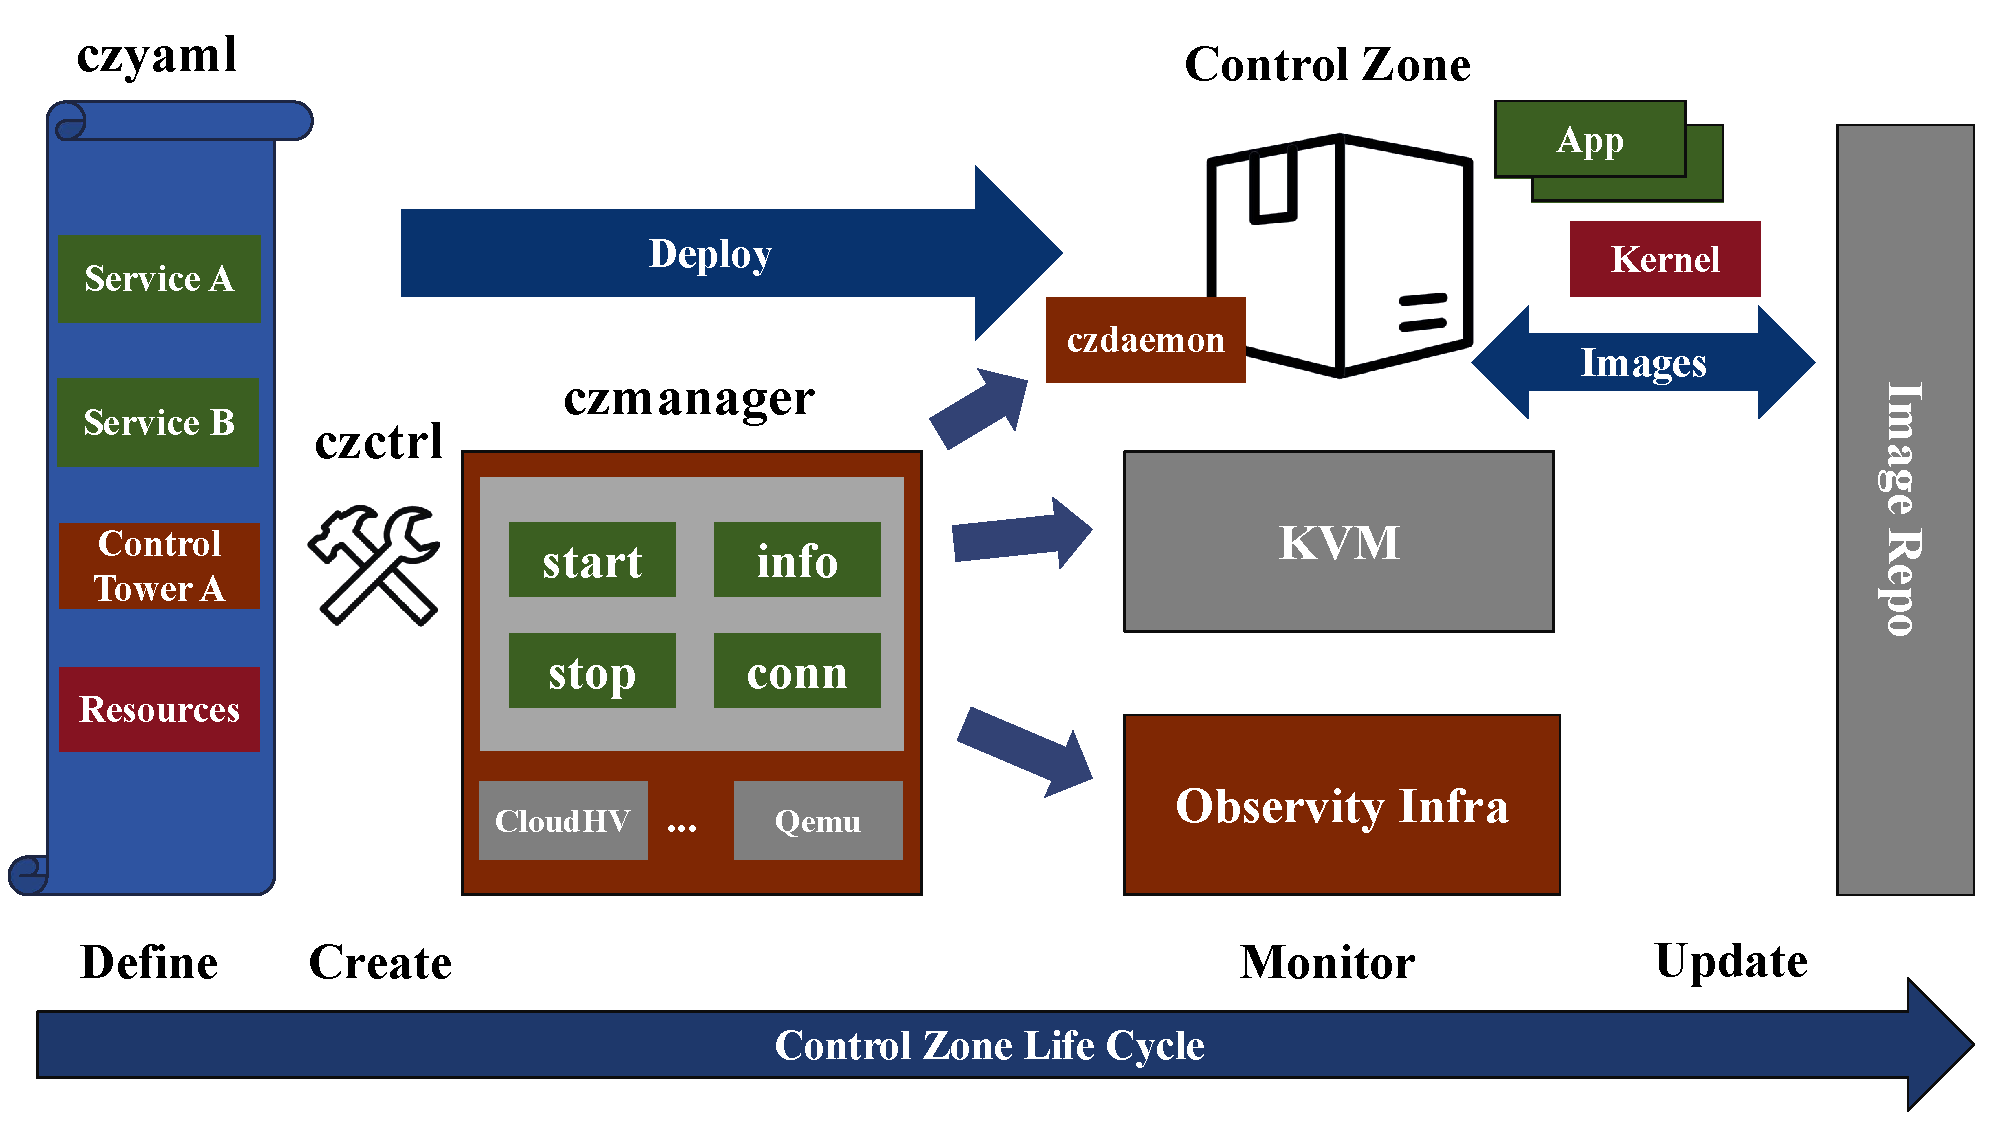
\includegraphics[width=0.9\textwidth]{cz_components}
    \bicaption{\quad Control Zone组件结构}{\quad Components of Control Zone}
    \label{fig:cz_components}
\end{figure}

czcli(Control Zone CLI)负责进行Control Zone的生命周期管理,也是Control Zone实现的核心一环。其主要与两个模块进行交互,Monitor是前文中实现的可观测基础设施,在本章用于对Control Zone的性能监控与服务的劣化监测。KVM是本文研究中所使用的虚拟化环境。czcli需要解析混部策略的配置,构造好沙箱环境,并按照策略中的定义运行相关的容器。不同于与常见的Docker等容器沙箱,Control Zone会对容器中部分资源配置进行特殊处理:

1)所有与资源有关的声明,都会转化为虚拟机资源的声明,通常会设置为所有混部应用所需求的资源加总,同时,Control Zone也支持对于LLC与内存带宽等其他硬件资源的质量要求声明,czcli会额外地在Intel RDT子系统中创建对应的条目来满足应用对此类资源的需求。

2)考虑到要对混部应用的QoS进行监测,因此网络相关的声明会被czcli特殊处理,通常是转化为envoy的配置,从而使得混部应用的流量会通过envoy代理,进而实现对于应用QoS的监测,默认情况下envoy提供L3-L4层的基本网络监测,Control Zone配置中也指明应用的类型来获取L7等更高层次的QoS监测。

\section{Control Zone管理流程}

启动Control Zone的流程如图~\ref{cz_start}所示,czcli首先会对配置进行检验,随后生成虚拟机及要运行容器的相关配置,其中虚拟机配置通过libvirt接口请求KVM创建目标虚拟机,等待虚拟机启动完毕之后,首先按配置中的容器启动要求先后启动调度器与混部容器,在这过程中,对于虚拟机的监控会伴随虚拟机的启动而开始,而对于服务的QoS监控则会等到所有容器都启动完毕后再开始。

\begin{figure}[!htbp]
    \centering
    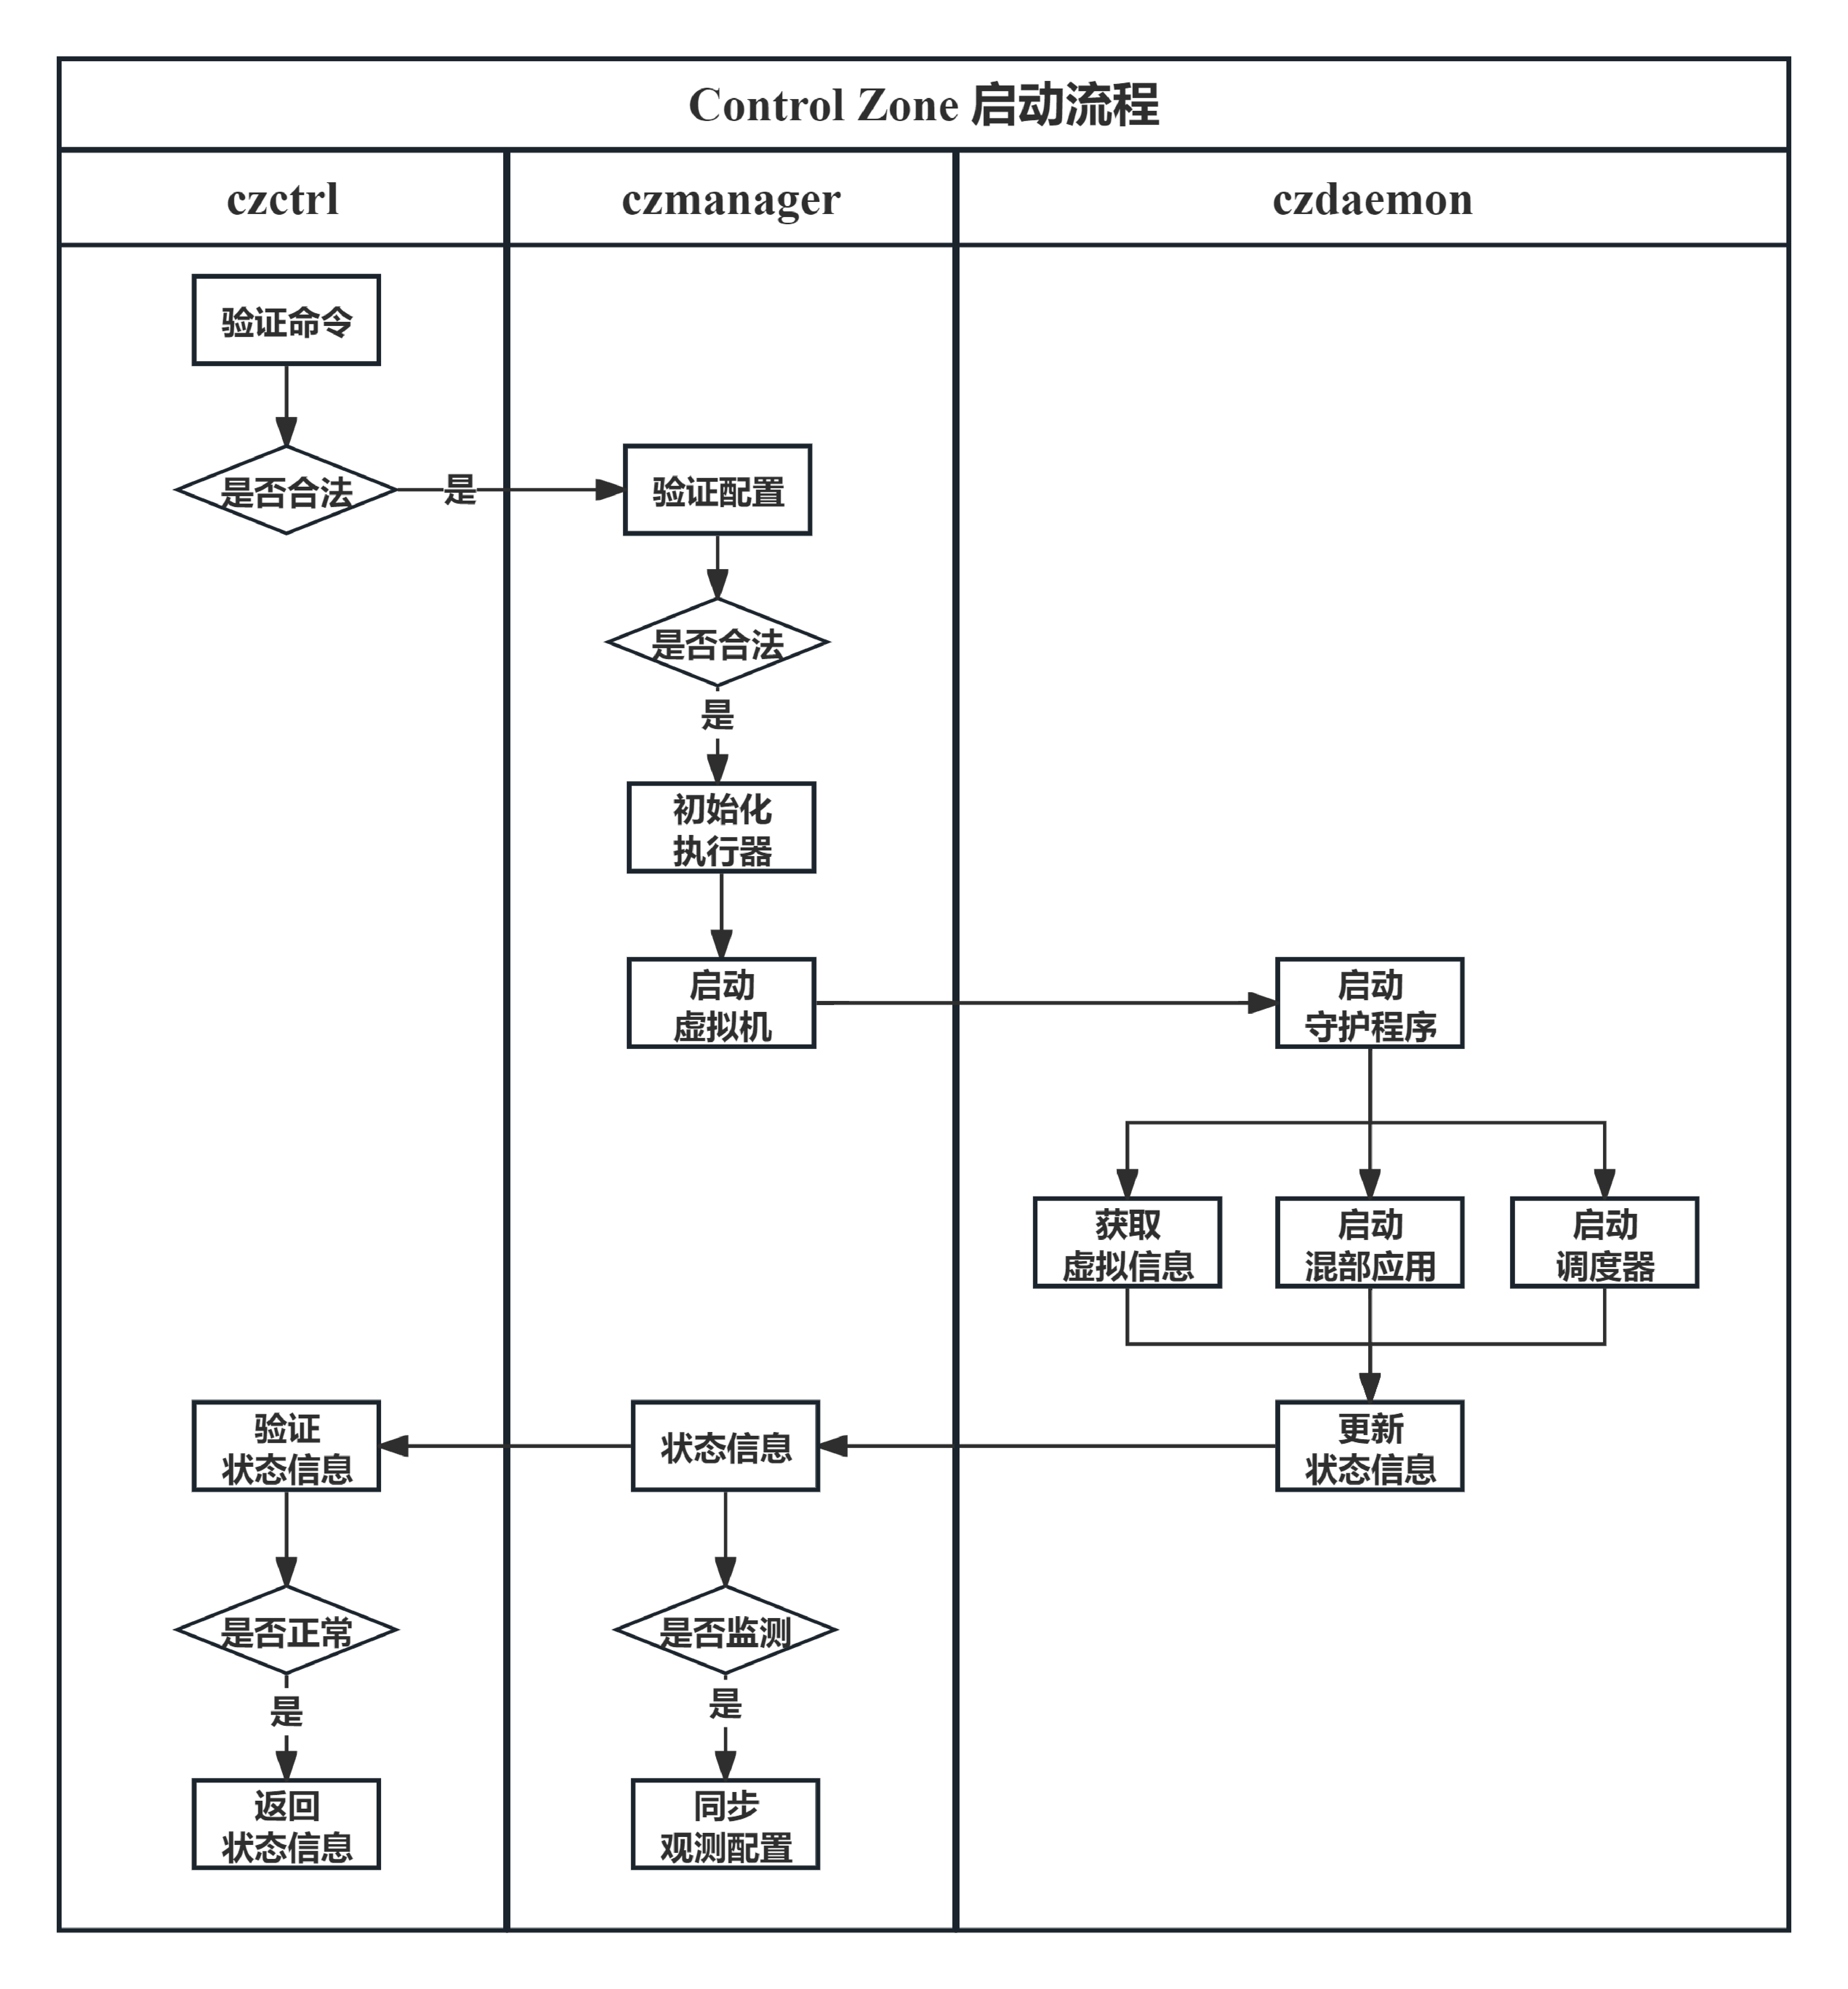
\includegraphics[width=0.7\textwidth]{cz_start}
    \bicaption{\quad Control Zone启动流程}{\quad Control Zone Starting}
    \label{fig:cz_start}
\end{figure}

更新Control Zone的流程如图~\ref{cz_update}所示,czcli同样会验证相关配置,并根据所要修改的内容, 按照虚拟机、调度器、混部容器的顺序依次进行配置的更新。

\begin{figure}[!htbp]
    \centering
    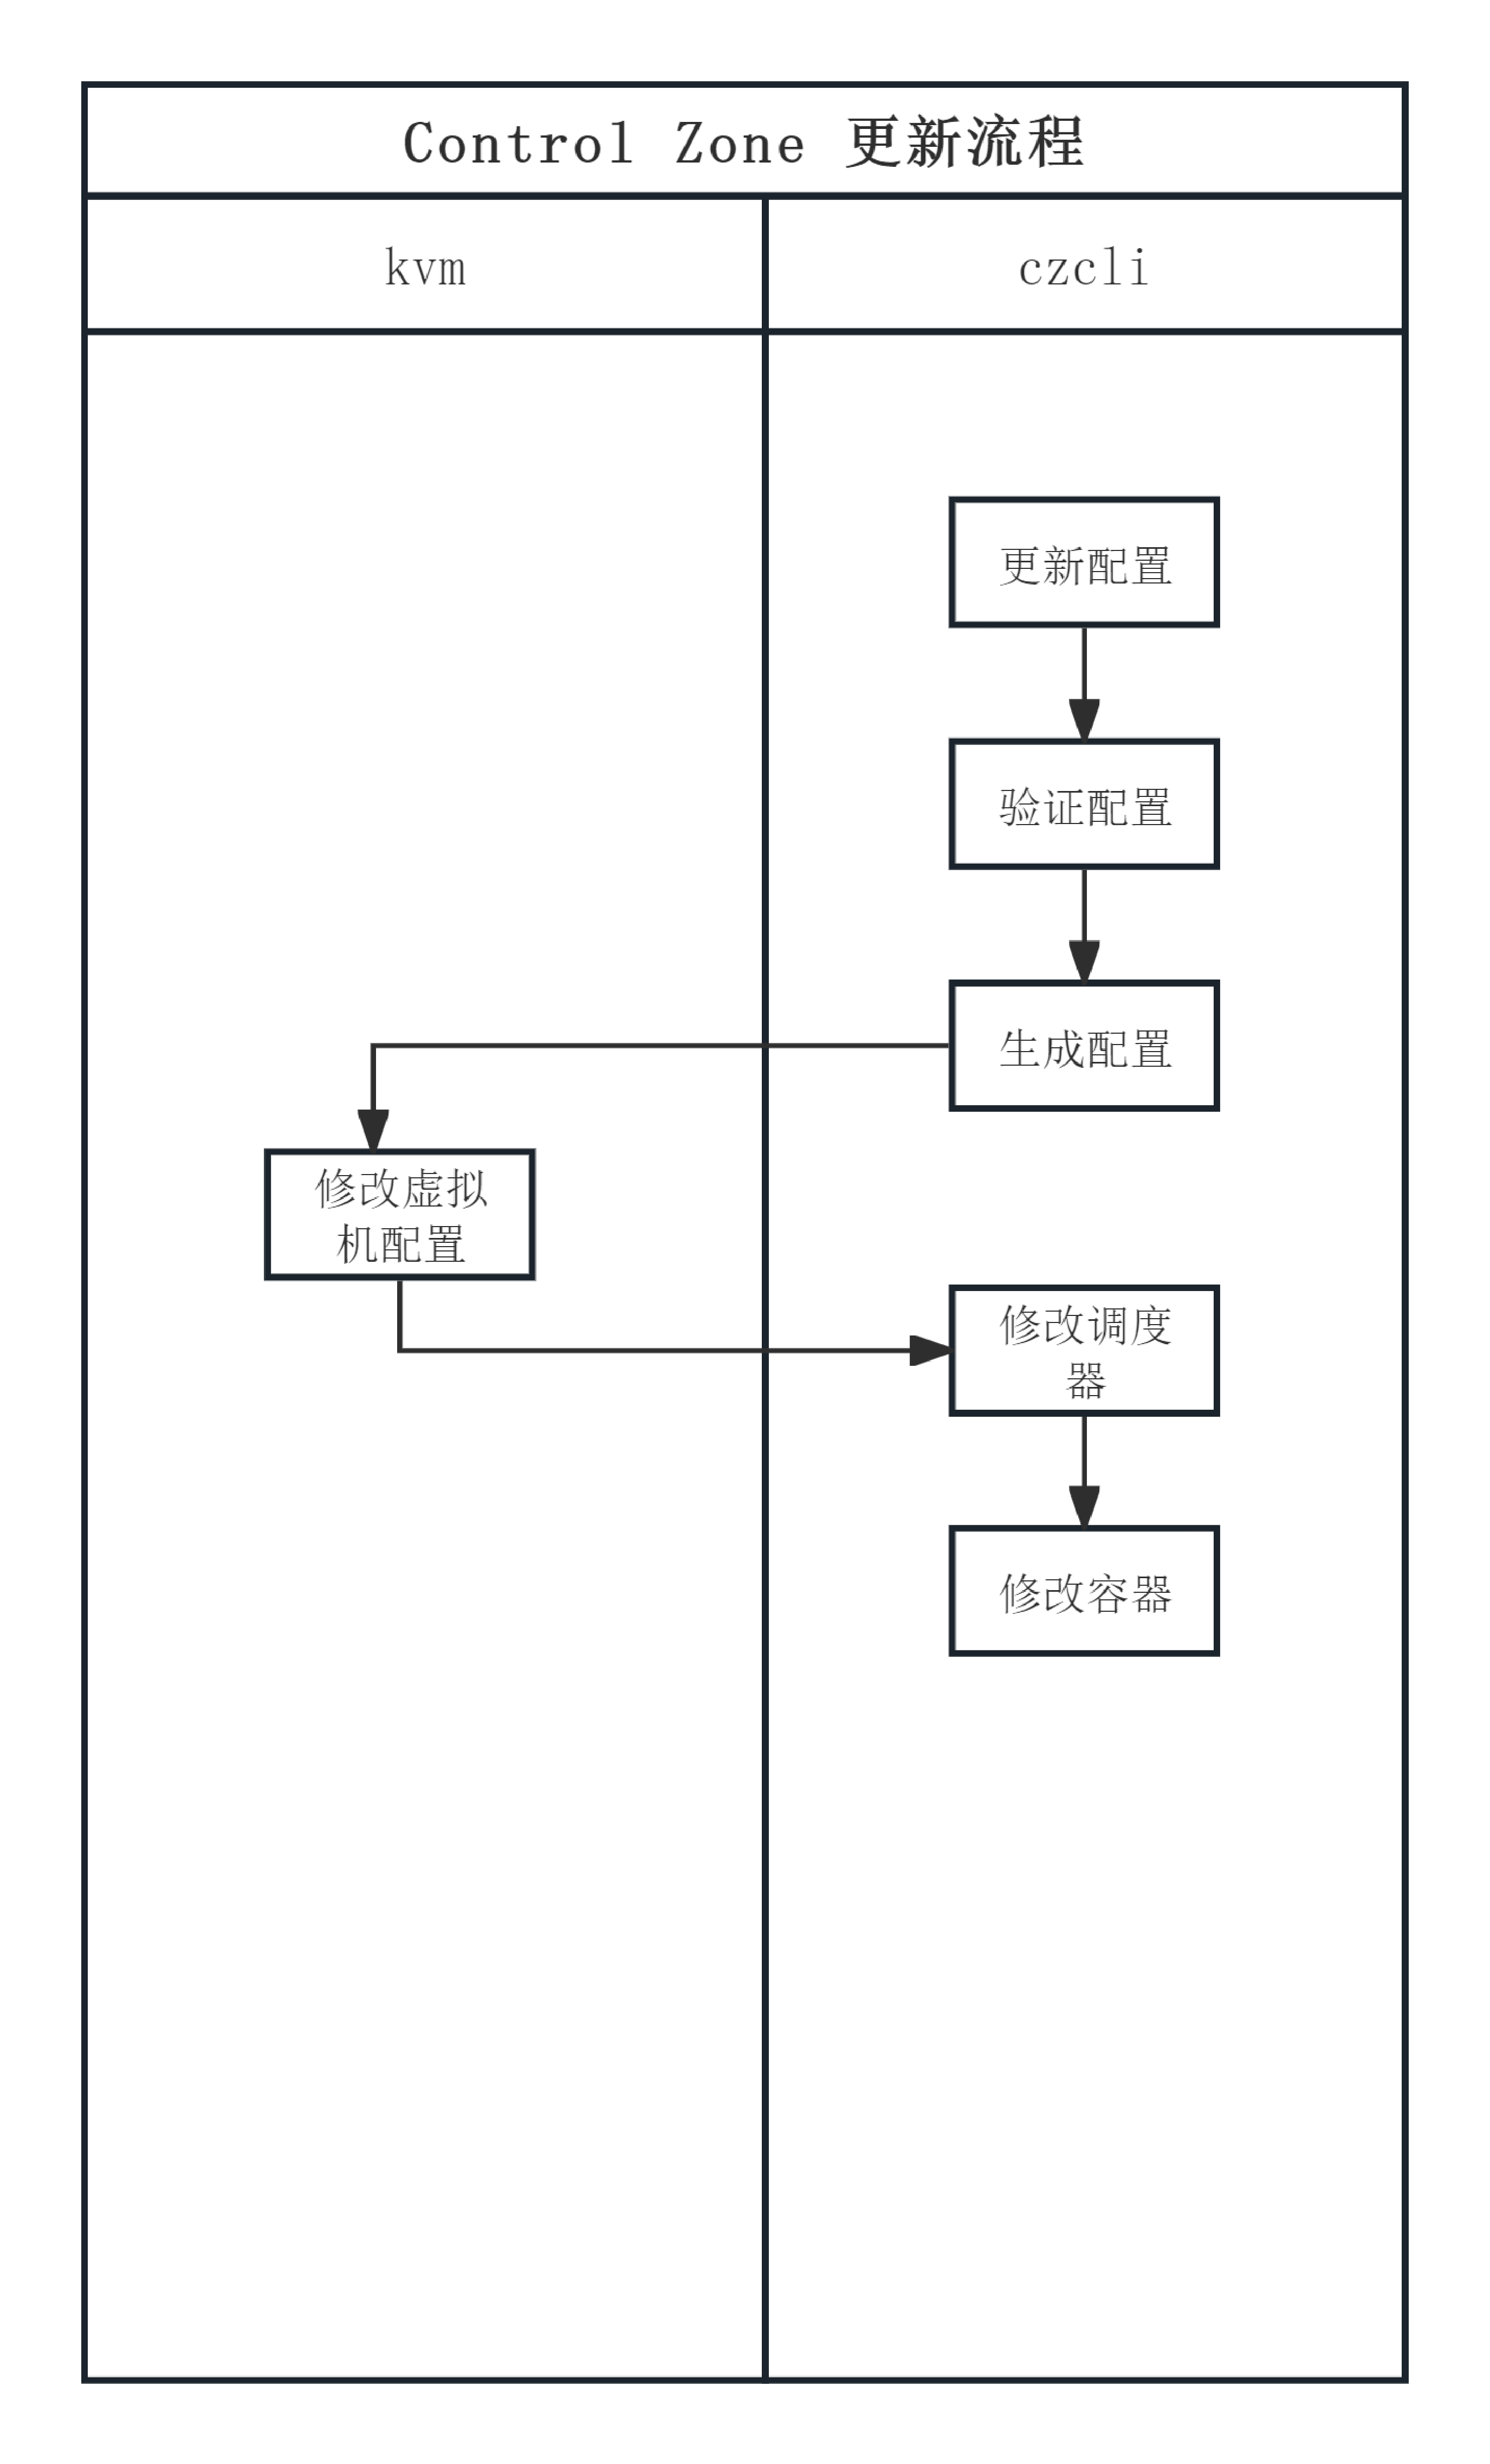
\includegraphics[width=0.7\textwidth]{cz_update}
    \bicaption{\quad Control Zone更新流程}{\quad Control Zone Updating}
    \label{fig:cz_update}
\end{figure}

回收Control Zone的流程如图~\ref{cz_update}所示,czcli首先会根据配置判断Control Zone是否存在,然后按照与启动相反的顺序,首先关闭混部容器,同时停止相关的服务监控,然后卸载调度容器,当所有业务相关容器均关闭时,首先停止对Control Zone的性能监控, 最后再回收其他资源并关闭虚拟机。

\begin{figure}[!htbp]
    \centering
    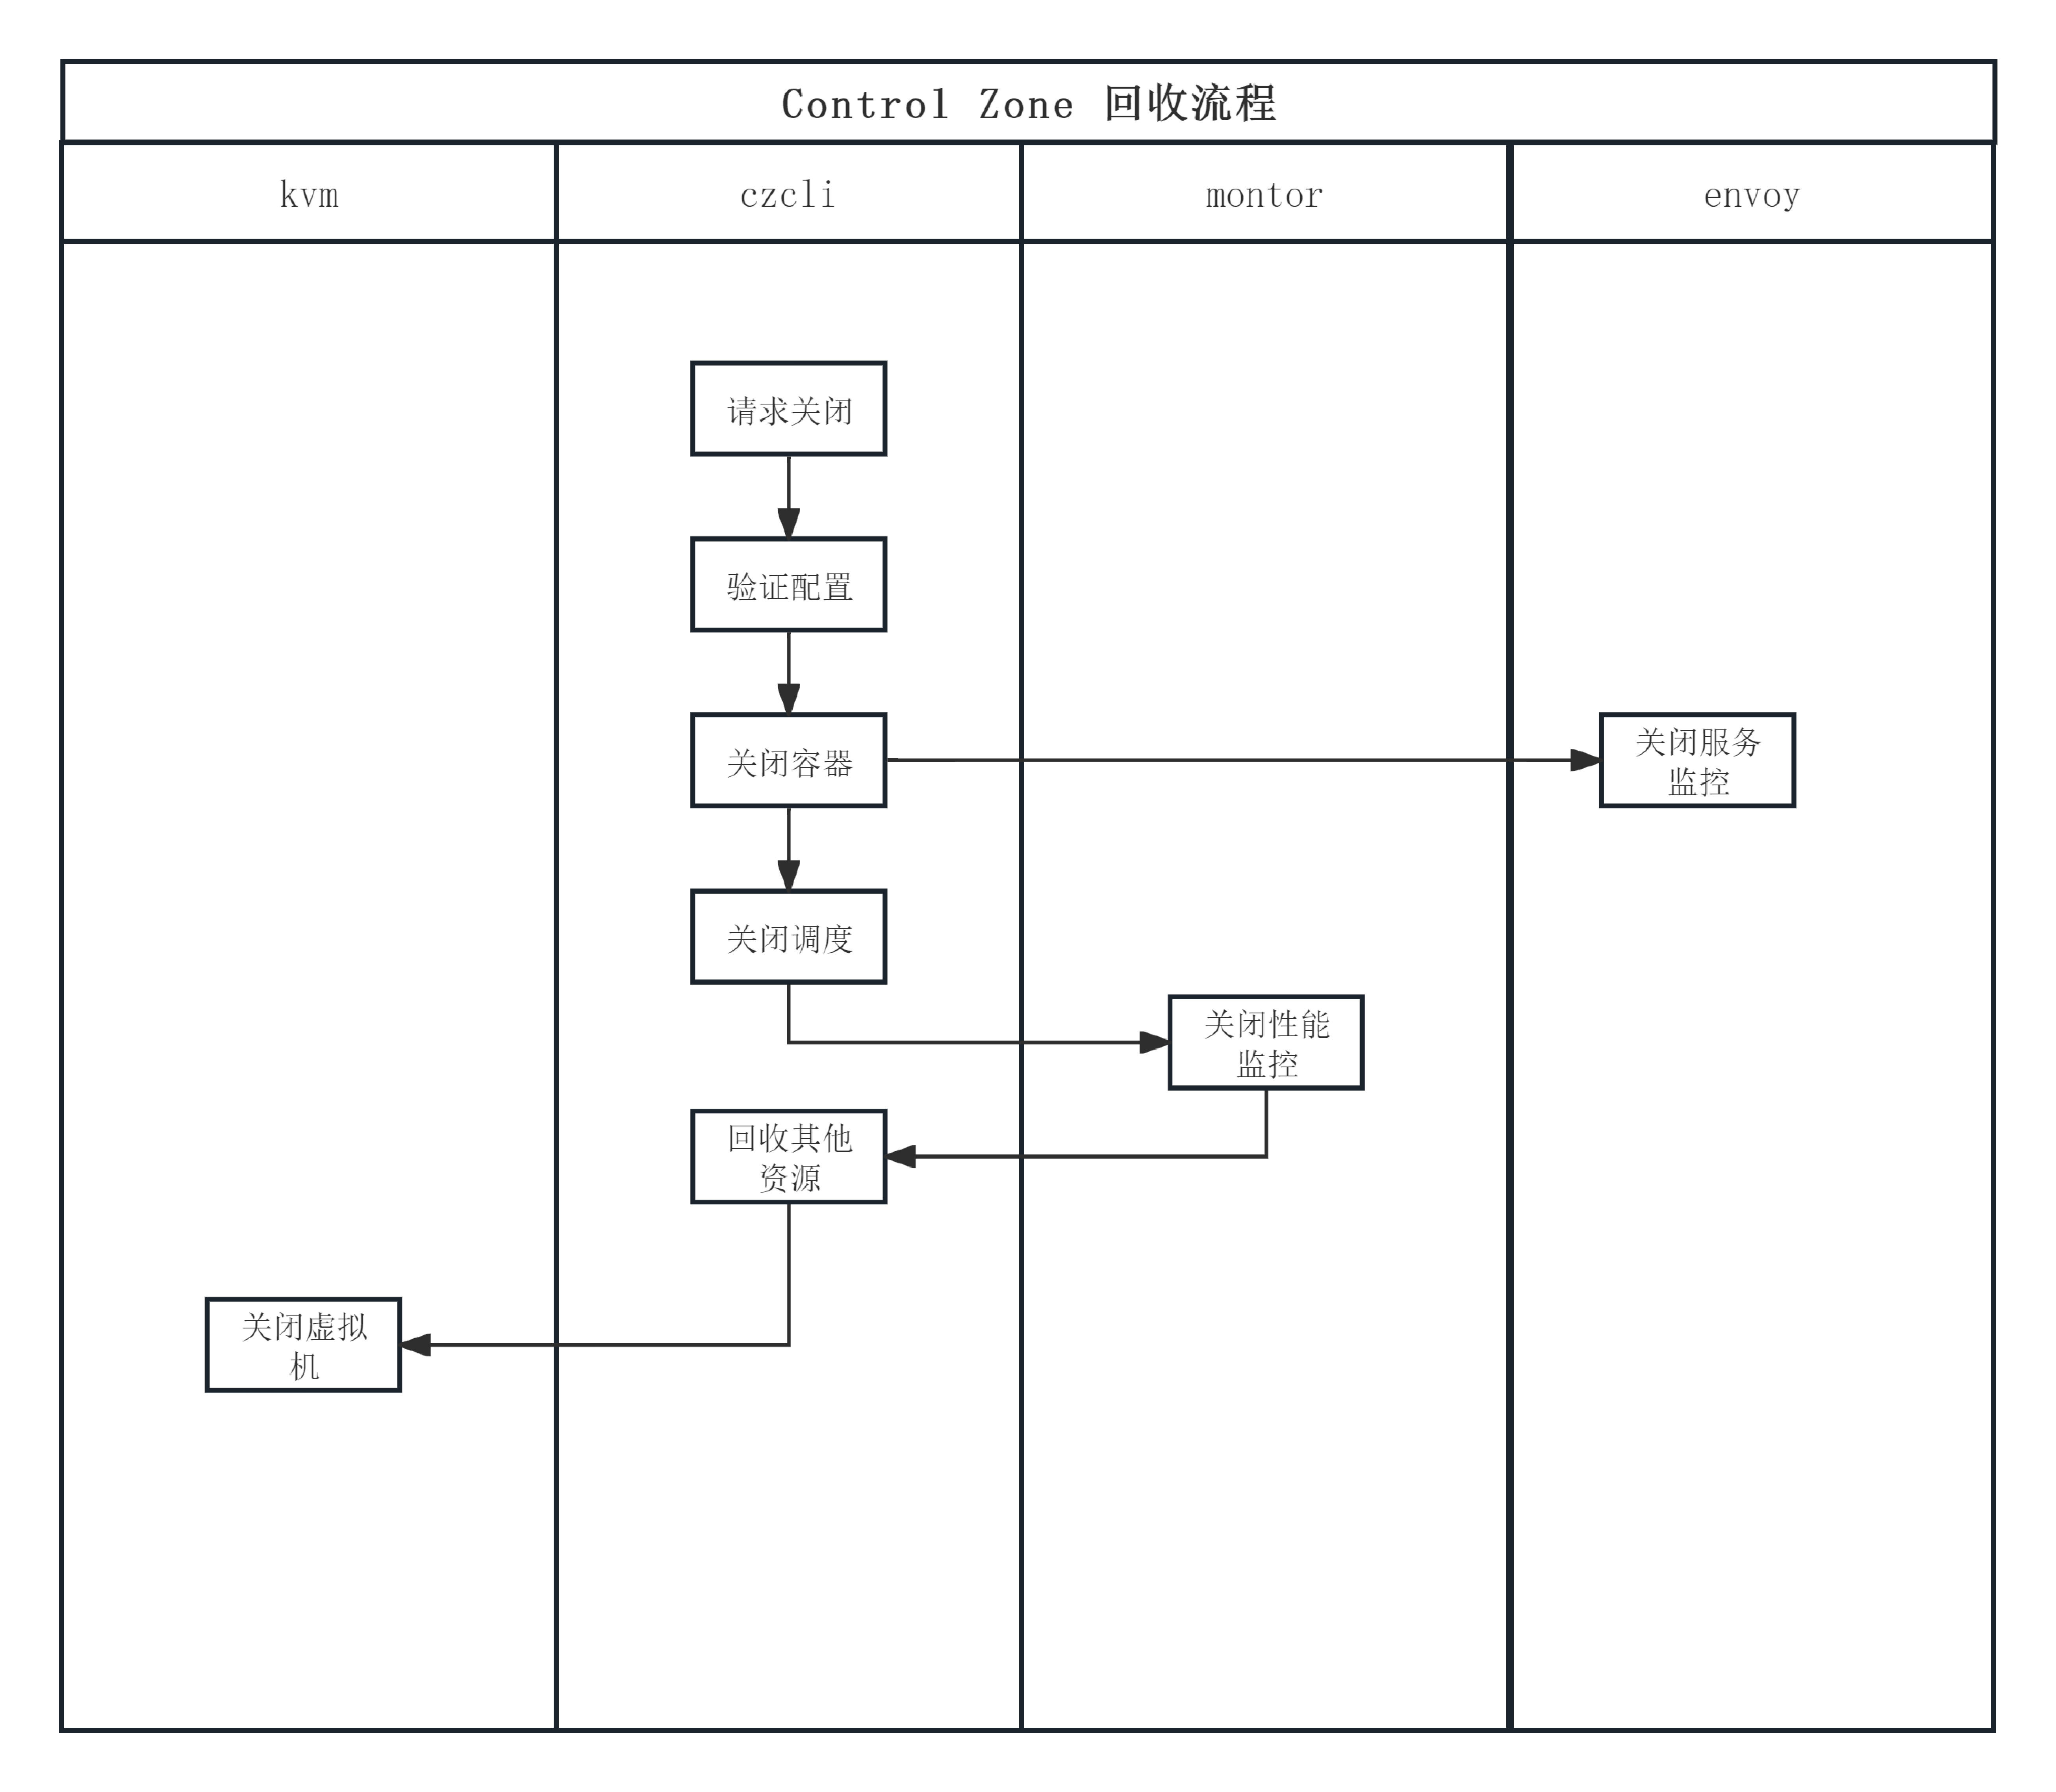
\includegraphics[width=0.7\textwidth]{cz_end}
    \bicaption{\quad Control Zone回收流程}{\quad Control Zone Destroying}
    \label{fig:cz_end}
\end{cz_end}

\section{本章小结}

本章首先介绍了运行时调度可变的沙箱Control Zone的实现,然后再对其生命周期中的各个流程进行分析。Control Zone通过虚拟机粒度的沙箱,增强了不同混部方案之间的隔离性,同时在同一个沙箱中,允许设置自定义的调度策略。除提供沙箱这样基本的功能以外,Control Zone还提供了了一套性能监控与劣化监测的机制,用于为后续调度提供信息辅助。